\section{Introduction}
\label{intro}
\subsection{Wave Energy Overview}
%(Why WECs, in renewable energy context):

% stronger opening sentence
The global climate crisis requires a transition to carbon-free energy sources such as ocean wave energy.
Ocean waves have higher consistency, predictability, and energy density than other renewable energy sources such as wind and solar, while the temporal complementarity of waves with other resources can improve grid resilience and capacity adequacy, decrease energy prices, and decrease requirements for energy storage and balancing power \cite{akdemir_opportunities_2023,bhattacharya_timing_2021,pennock_temporal_2022}.
Wave energy converters (WECs), the devices that harness and convert this energy, could provide both electricity for the grid at large scale and power for smaller offshore technologies like aquaculture, desalination, and marine sensing \cite{PBE}.
Despite the potential advantages of WECs, a significant decrease in the cost per unit energy production is required before the technology can be deployed at large scales. %\hl{(Add a more specific number to show that the LCOE needs to come down an order of magnitude).} Meanwhile, a lack of design convergence (...)
Thus, a design process that emphasizes techno-economic viability from an early stage is necessary.

%(Why multidisciplinary):
However, the presence of strong interdisciplinary coupling complicates the application of typical design and optimization techniques to WECs.
The powertrain, controller, bulk dimensions, hydrodynamic shape, and structural thicknesses must be selected to balance the complex tradeoff between power production and cost while ensuring survivability and practical feasibility.
Concentrating and automating the design decision-making efforts of structural, control, hydrodynamics, and electrical engineers while accurately capturing all major relationships and requirements is challenging, not to mention computationally prohibitive.
Nonetheless, leveraging the coupling between subsystems and across technical domains can produce large gains in techno-economic viability.
Automating this process through optimization allows WEC designers to more quickly and systematically explore tradeoffs of major design decisions, and could eventually allow standardized comparisons between different WEC architectures.
Thus, performing a system-level WEC optimization that simultaneously considers the coupled techno-economic goals, design decisions, and requirements is highly advantageous.
%Figure~\ref{fig:disciplines} is a non-exhaustive outline of the most common disciplines in a wave energy converter, and the level and direction of coupling between them.

% what is RM3
An initial attempt to consolidate a multidisiplinary WEC design process, though without optimization, was the Reference Model Project.
From 2010 to 2014, the U.S.
Department of Energy funded the creation of six benchmark designs for marine energy devices, published a report \cite{RM3} describing the design considerations and performance calculations, and released design artifacts and other documentation on its website.\footnote{\url{https://openei.org/wiki/PRIMRE/Signature_Projects/Reference_Model}} Three designs are for tidal and current energy turbines, and three are WECs.
The third reference model, known as RM3, is a two-body point absorber WEC designed for a reference site located in Humboldt Bay, California.
The major structural components of the device are a surface float and a spar consisting of a vertical column and a subsurface damping plate, shown in Figure \ref{fig:rm3-parts}.
The float oscillates up and down with oncoming incident waves while the spar stays mostly stationary, and electrical power is produced from this relative heave motion.
\begin{figure}[!ht]%% placement specifier
\centering%% For centre alignment of image.
\includegraphics[width=1\linewidth]{\matlabFilepath{1}}
\caption{RM3 geometry visualized}\label{fig:rm3-parts}
\end{figure}
RM3 has received considerable research attention in the decade since the original report was published.
The present study builds on that work and presents a multidisciplinary techno-economic simulation of the RM3.

The remainder of the introduction will review WEC system modeling literature, articulate the appeal of semi-analytical modeling to address gaps in the field, and identify the paper's key contributions and structure.

\subsection{WEC System Modeling: State of the Art and Gaps}
\label{sec:lit}

% design optim / concurrent design in industry
Before reviewing the academic state of the art in WEC multidisciplinary modeling, it is worth evaluating the popularity of concurrent design practices in the wave energy industry.
\cite{trueworthy_wave_2020} provides a critical summary of the WEC design process and shares survey results from 25 WEC designers and developers.
50\% of respondents design all subsystems concurrently.
The others tend to start with the WEC shape and PTO, then move to the controller and moorings, and finish with the power transportation system.
\cite{trueworthy_wave_2020} concludes that concurrent design has promise to take advantage of subsystem interactions and is an under-utilized technique worthy of further study, emphasizing the importance of incorporating all design requirements at an early stage.

% review papers on wec optim

Other references outline relevant guidelines for WEC survivability design without a formal optimization procedure \cite{coe_survey_2018, ove_arup__partners_ltd_structural_2016,paduano_towards_2024,giannini_wave_2022}.

% table summary
Moving on to specific optimization studies, table~\ref{tab:lit} compares the modeling and optimization formulations of a variety of the most relevant examples.
A wide variety of WEC optimizations have been conducted.
After first examining the overall trends, each table entry will be described in more detail.
Point absorbers (PA) seem to be the most common device architecture, though most major device types are represented, and several studies optimize arrays of multiple devices.
Nearly all model hydrodynamics and power production in some way.
Hydrodynamic modeling is typically performed with the boundary element method (BEM), occasionally with semi-analytical models like matched eigenfunction expansion method (MEEM), and rarely with high fidelity CFD.
Dynamic modeling is frequently performed both in the frequency domain (F) and time domain (T), with a handful of studies using extensions of frequency domain techniques (F+) to handle constraints and nonlinearities that are typically only handled in the time domain, and a few using the newer pseudo-spectral method (PS).
A range of controllers are considered, including proportional-integral / reactive (PI), proportional / pure damping (P), their extensions to incorporate constraints (P+/PI+), nonlinear structured (NL), and unstructured (UNS).
Optimizations that incorporate powertrain, structures, and economics are less of a guarantee but still common, while incorporating mooring is relatively rare.
Each discipline may be incorporated with varying levels of fidelity.
It is most common to simulate irregular waves (IRR), though several assume regular waves (REG).
Several incorporate multiple sea states through the use of a joint probability density matrix (IRR+/REG+), and only a few consider storm sea states (STO).
Optimizers used include numerical optimization algorithms like genetic algorithms (GA) and local optimizers (LOC), analytical optimization via Pontryagin's maximum principle (PMP), as well as non-optimization techniques such as design of experiments (DOE), manual iteration (IT), and brute force sweeps (BF).
Objectives are usually power (PWR) or a measure of economic viability or proxy thereof (ECON).
Less common objectives include measures of power variability (VAR), array interaction (ARRY), load (LO), and bandwidth (BW).
The constraints column describes all the requirements the designs are made to satisfy, whether this is achieved with actual optimization constraints or by the simulation model.
Constraint categories include device geometry (GEO), motion amplitude (AMP), the power take-off (PTO), dynamic stability (STA), structural failure (STR), and power (PWR).
The design variables column counts only the optimization decision variables corresponding to an actual design parameter, and not any state variables that may be included in the optimization decisions, such as in the direct transcription or pseudospectral formulations.
Common design variables are bulk dimensions (DIM), hull shape (SHP), and control parameters (CTL).
PTO design variables are common among the pseudo-spectral optimizations, while structural (STR) design variables are rare.
Most studies have fewer than five design variables, with the three largest optimizations having 14, 15, and 66 variables.

%Need to copy sources over from slide 27 and 35 of F24 reseach slides with original charts (with color)

\begin{longtable}{
    >{\centering\arraybackslash}p{0.03\linewidth}|
    >{\centering\arraybackslash}p{0.07\linewidth}|
    >{\centering\arraybackslash}p{0.072\linewidth}|
    >{\centering\arraybackslash}p{0.040\linewidth}|
    >{\centering\arraybackslash}p{0.019\linewidth}|
    >{\centering\arraybackslash}p{0.025\linewidth}|
    >{\centering\arraybackslash}p{0.059\linewidth}|
    >{\centering\arraybackslash}p{0.059\linewidth}|
    >{\centering\arraybackslash}p{0.059\linewidth}|
    >{\centering\arraybackslash}p{0.059\linewidth}|
    >{\centering\arraybackslash}p{0.072\linewidth}|
    >{\centering\arraybackslash}p{0.072\linewidth}}
\rot{\textbf{Ref}} & \rot{\textbf{Device}} & \rot{\textbf{Hydro}}& \rot{\textbf{Drag}} & \rot{\textbf{\# DOF}} & \rot{\textbf{Domain}} & \rot{\textbf{Controls}} & \rot{\textbf{Mooring}} & \rot{\textbf{Powertrain}} & \rot{\textbf{Structures}} & \rot{\textbf{Economics}} & \rot{\textbf{Sea state}} \\
\hline
This work & 2-PA & MEEM & DF & 1 & F+ & PI+ & - & EFF & AN & STR, PTO & REG+, STO \\

\cite{mccabe_multidisciplinary_2022} & 2-PA & ALG & - & 1 & F+ & PI+ & - & EFF & AN & STR & REG+, STO \\

\cite{khanal_multi-objective_2024} & 1-PA array & BEM & - & 4 & F & PI+ & - & - & - & GEO & REG \\

\cite{gaudin_single_2021} & 1-PA array & MEEM & - & 120 & F & PI & DES & - & AN & MOOR & IRR+, STO \\

\cite{edwards_optimisation_2022} & 1-PA & BEM & - & 1 & F & P & - & - & - & GEO & REG \\

\cite{garcia-teruel_reliability-based_2021}& 1-PA & BEM & LD & 1 & F+ & PI & - & - & LD & - & IRR+ \\

\cite{garcia-teruel_design_2022}& 1-PA & BEM & - & 2 & F+ & PI & - & - & - & - & IRR \\

\cite{cotten_multi-objective_2022} & ATN & BEM & - & 10 & F+ & P & - & - & LD & - & IRR+ \\

\cite{abdulkadir_control_2024} & 1-PA & MEEM & LD & 2 & T & NL P & - & - & - & - & IRR \\

\cite{housner_numerical_2024} & TRM & BEM & - & 4 & T & PI & DYN & - & - & - & REG \\

\cite{al_shami_parameter_2019} & 2-PA & BEM & DF & 2 & F & PI & - & - & - & - & REG \\

\cite{RM3} & 2-PA & BEM & Q & 2 & T & P & DES & - & FEA & FULL & IRR+, STO \\

\cite{mi_multi-scale_2025} & OSW & BEM & Various & 8 & T & PI & DYN, DES & DYN & FEA & FULL & IRR+, STO \\

\cite{an_optimal_2024} & OTP & CFD & CFD & - & T & - & - & - & FEA & - & STO \\

\cite{ambuhl_reliability-based_2014} & 1-PA & - & Q & - & - & - & DES & - & AN & STR & STO \\

\cite{nguyen_theoretical_2024} & OSW & MEEM & LD & 1 & F & PI & - & - & LD & - & IRR \\

\cite{ferri_balancing_2014} & 1-PA & BEM & LD & 1 & T & P, PI+, UNS & - & DYN & LD & STR & IRR+ \\

\cite{rosati_control_2023} & OWC & BEM & - & 1 & T & NL P+ & - & EFF & - & PTO & IRR+ \\

\cite{son_performance_2016} & 2-PA & MEEM & LD & 1 & F & P & - & EFF & - & - & REG \\

\cite{gaebele_tpl_2025} & 2-PA & BEM & - & 2 & PS & PI & - & DYN, EFF & - & PTO, GEO & IRR \\

\cite{devin_high-dimensional_2024} & 1-PA & FIT & - & 1 & PS & UNS & - & DYN, EFF & - & - & REG \\

\cite{grasberger_control_2024} & OSW & BEM & - & 1 & PS & PI & - & DYN & - & GEO & IRR \\

\cite{herber_dynamic_2014} & 1-PA & FIT & LD & 1 & T & UNS & - & - & - & - & IRR \\

\cite{lin_fast_2025} & 1-PA & BEM & LD & 1 & F+ & UNS & - & - & - & - & IRR+ \\

\cite{abdulkadir_optimal_2024} & 1-PA array & BEM & - & 3 & T & UNS & - & - & - & - & IRR \\

%\cite{zhang_performance_2024} & 3-PA & MEEM & LD & 3 & F & P & DYN & - & - & - & IRR
%& BF & PWR & - & CTL & 2 \\

%\cite{wen_shape_2018} & 1-PA & BEM & - & 1 & F & P & - & - & - & - & IRR+
%& DOE, LOC & PWR & STA & DIM, SHP & 3 \\

\hline 
\caption{Comparison of the disciplinary scope and modeling fidelity of previous WEC models used for optimization}
\label{tab:lit}
%\fillandplacepagenumber
\end{longtable}

\begin{landscape}
\begingroup
\begin{table}
    \centering
    \begin{tabular}{
        >{\centering\arraybackslash}p{0.065\linewidth}
        >{\raggedright\arraybackslash}p{0.13\linewidth}|
        >{\centering\arraybackslash}p{0.065\linewidth}
        >{\raggedright\arraybackslash}p{0.13\linewidth}|
        >{\centering\arraybackslash}p{0.065\linewidth}
        >{\raggedright\arraybackslash}p{0.13\linewidth}|
        >{\centering\arraybackslash}p{0.065\linewidth}
        >{\raggedright\arraybackslash}p{0.11\linewidth}|
        >{\centering\arraybackslash}p{0.065\linewidth}
        >{\raggedright\arraybackslash}p{0.13\linewidth}}
         \multicolumn{2}{c|}{Device}&  \multicolumn{2}{c|}{Hydro}&  \multicolumn{2}{c|}{Drag} &\multicolumn{2}{c|}{Domain} & \multicolumn{2}{c}{Controls} \\ \hline
         N-PA&  N-body floating point absorber&  MEEM&  Matched eigenfunction expansion method or similar &  DF& Describing function & F&Frequency domain & P&Proportional (pure damping) \\
         ATN&  Attenuator&  BEM&  Boundary element method&  LD& Linear damping & F+&Frequency domain extension & PI&Proportional integral (damping and stiffness, aka reactive) \\
         TRM&  Terminator&  CFD&  Computational fluid dynamics&  Q& Quadratic & T&Time domain & P+, PI+&P/PI control extended to incorporate constraints \\
         OSW&  Oscillating surge WEC&  FIT&  Fit of model to numerical or experimental data&  CFD& Computational fluid dynamics & PS&Pseudo-spectral& NL&Nonlinear structured \\
         OTP&  Overtopping&  ALG&  Algebraic approximation&  &  & & & UNS&Nonlinear unstructured \\
        OWC& Oscillating water column& & & & & & & & \\
    \end{tabular}
    \caption{Legend keys for the dynamics and controls columns of table~\ref{tab:lit}}
    \label{tab:lit-review-legend-dynam}
\end{table}
\endgroup
\end{landscape}

\begin{landscape}
\begingroup
\begin{table}
%    \centering
    \begin{tabular}{>{\centering\arraybackslash}p{0.05\linewidth}>{\raggedright\arraybackslash}p{0.2\linewidth}|>{\centering\arraybackslash}p{0.05\linewidth}>{\raggedright\arraybackslash}p{0.2\linewidth}|>{\centering\arraybackslash}p{0.05\linewidth}>{\raggedright\arraybackslash}p{0.2\linewidth}|>{\centering\arraybackslash}p{0.05\linewidth}>{\raggedright\arraybackslash}p{0.2\linewidth}}
         \multicolumn{2}{c|}{Mooring}& \multicolumn{2}{c|}{Structures} &  \multicolumn{2}{c|}{Economics}&  \multicolumn{2}{c}{Sea state}\\ \hline
         DYN&  Model incorporates mooring dynamics &  AN&  Models stress analytically as a function of dimensions&  STR&  Models structural cost &  REG
& Regular waves\\
         DES&  Study considers mooring physical design &  LO&  Models load without dimension-dependent stress &  PTO&  Models power take-off cost &  IRR
& Irregular wave spectrum\\
         &  &  FEA&  Models stress using finite element analysis &  GEO&  Geometric cost proxy (i.e. hull volume, surface area)&  REG+, IRR+& Joint probabilities of wave heights and periods for multiple sea states\\
         &  &  &  &  FULL&  Full cost model &  STO& Storm condition\\
    \end{tabular}
    \caption{Legend keys for other modeling columns of table~\ref{tab:lit}}
    \label{tab:lit-review-legend-other}
\end{table}

\endgroup
\end{landscape}


% Prior WEC optimization across discipline
More specifically, a few studies \cite{gaudin_single_2021,khanal_multi-objective_2024,edwards_optimisation_2022,garcia-teruel_reliability-based_2021} perform WEC optimization with several disciplines.
These studies are notable for their large scales of 120 degrees of freedom and 14, 15, and 66 design variables respectively.
\cite{gaudin_single_2021} optimizes an array of 20 submerged cylinders, holding the WEC design constant but optimizing site selection, array layout, and mooring design while considering cable and pile cost as well as pile load capacity.
\cite{khanal_multi-objective_2024} optimizes an array of four cylindrical point absorbers, with 4 modeled disciplines of array layout, hydrodynamics, controls, and economics.
\cite{edwards_optimisation_2022} is a point absorber shape optimization study that minimizes surface area as a cost proxy, accounts for stability constraints, and considers only geometries with power extraction equal to theoretical radiation, amplitude, and steepness limits.
\cite{garcia-teruel_reliability-based_2021}, along with the smaller scale study \cite{garcia-teruel_design_2022} by the same authors, apply multi-objective optimization to trade off power with fatigue load and device volume, respectively.
\cite{cotten_multi-objective_2022} similarly optimizes fatigue load for an attenuator-style WEC with many more degrees of freedom but fewer (8) design variables.
A different 8-variable shape optimization \cite{abdulkadir_control_2024} notably calculates hydrodynamic coefficients via the semi-analytical matched eigenfunction expansion method (MEEM), rather than from boundary element method as is typical, but does not include disciplines beyond hydrodynamics and dynamics/controls.

Regarding optimization algorithm, all seven of these studies \cite{khanal_multi-objective_2024,gaudin_single_2021,edwards_optimisation_2022,garcia-teruel_reliability-based_2021,garcia-teruel_design_2022,cotten_multi-objective_2022,abdulkadir_control_2024} utilize the genetic algorithm, a population-based heuristic method.
The alternative to heuristic methods is local optimization, which lacks the exploratory capability of heuristic methods to avoid getting stuck in local optima, but beneficially leverages any smoothness in the objective and scales well to a large ($>50$) number of design variables \cite{martins_engineering_2022}.
A team at NREL attempted local optimization for a terminator shape study but found they could only reasonably optimize 3 of the intended 13 design variables at a time due to the high computational cost of their time-domain simulation \cite{housner_numerical_2024}.
The previous studies \cite{garcia-teruel_reliability-based_2021,garcia-teruel_design_2022,cotten_multi-objective_2022} avoided this issue by simulating primarily in the frequency domain and using the time domain only to address PTO constraints.
Alternatively, design-of-experiment techniques enable systematic exploration of the design space without the use of traditional optimizers.
For example, \cite{al_shami_parameter_2019} performs a 7 design variable shape optimization with the Taguchi method.

Structural optimization of WECs faces a similar challenge in the high compute time of finite element analysis (FEA).
FEA of WECs is most often performed with manual design iterations, as in \cite{RM3,mi_multi-scale_2025}.
These two studies, while not optimization, are extremely multidisciplinary, encompassing mooring design and detailed economic evaluation in addition to the more common hydrodynamics, powertrain, controls, and structures.
Automating the design process reported there remains a long term vision for WEC MDO.
Notably, one study \cite{an_optimal_2024} performs true optimization of WEC structural FEA using the commercial computer aided engineering software Altair Inspire.
The study examines four design variables, although it keeps the power calculations entirely separate from the structural optimization, neglecting the interdisciplinary coupling.
Another structural optimization does not consider power at all, but is able to perform a brute-force sweep of 3 design variables by using analytical equations for stress and other failure modes \cite{ambuhl_reliability-based_2014}.
Finally, several studies consider structures indirectly by examining the load on the device rather than the stress, e.g. \cite{nguyen_theoretical_2024, ferri_balancing_2014}, or equivalently assuming that stress scales with load and does not depend on any other dimensional design variable, e.g. \cite{garcia-teruel_reliability-based_2021, cotten_multi-objective_2022}.
Like the earlier MEEM study, \cite{nguyen_theoretical_2024} uses the equivalent analytical hydrodynamics in elliptical coordinates for an oscillating surge WEC.

The study \cite{ferri_balancing_2014} is notable because in addition to structural loads, it compares various control schemes and simulates second-order drivetrain dynamics.
The control co-design (CCD) methodology \cite{garcia-sanz_control_2019} emphasizes the importance of considering drivetrain dynamics and generator efficiency due to their strong effect on electrical power generation \cite{coe_useful_2023}.
A number of recent studies \cite{rosati_control_2023,son_performance_2016,anderson_re-imagining_2024,devin_high-dimensional_2024,grasberger_control_2024} simultaneously optimize the PTO with the controller.
\cite{rosati_control_2023} optimizes an OWC and is notable for its comparatively detailed cost modeling and its optimization of both economic and power variability metrics.
\cite{mccabe_multidisciplinary_2022} also optimized power variation, although that study's use of regular waves makes the variation formulation less useful.
Meanwhile, one point absorber PTO optimization \cite{son_performance_2016} is additionally notable for its use of the MEEM method.
\cite{gaebele_tpl_2025} is relevant because it optimizes the dimensional scale and PTO of the RM3 WEC directly using a control co-design approach.
It also efficiently incorporates many time-domain constraints (maximum force, speed, average power, RMS torque, and stroke) while maintaining frequency-domain hydrodynamics via the pseudo-spectral (PS) method, which \cite{devin_high-dimensional_2024,grasberger_control_2024} also use.
\cite{devin_high-dimensional_2024} completes a brute-force PTO optimization with 5 design variables, the highest of any brute force optimization considered here.
This is possible because instead of a five-dimensional sweep, the authors perform ten two-dimensional sweeps around a starting point obtained from an initial monte carlo design-of-experiments.
Finally, \cite{grasberger_control_2024} performs an outer brute-force sweep of two geometric design variables and an inner local optimization of 5 PTO and control design variables for an oscillating surge WEC. 

Other CCD papers optimize WEC dimensions without modeling the PTO.
\cite{herber_dynamic_2014} performs a direct transcription co-optimization of cylinder draft and radius with control.
\cite{lin_fast_2025} introduces a new CCD formulation for constrained control that is even faster than PS.
The method leverages the analytical Pontryagin Maximum Principle (PMP) and performs a case study to optimize a single geometric variable.
A different PMP formulation \cite{abdulkadir_optimal_2024} incorporates PTO-constrained array dynamics, although it has not yet been used for design optimization. 

% results / findings of the work
The results of prior studies provide insight into the level of improvement available with optimization and potential trends in the optimal design.
\cite{edwards_optimisation_2022} found that the axisymmetric geometry with minimum surface area and maximum power is a diamond-like shape that flares out just below the waterline and then back in.
\cite{devin_high-dimensional_2024} found that impedance matching at resonance has a large effect on power and PTO sizing has little effect.
This suggests that if cost were included, it may be preferable to have an undersized PTO that frequently saturates its control force.
This agrees with the conceptual argument of \cite{coe_maybe_2021} and the numerical findings of \cite{mcgilton_optimal_2024}.
The latter shows that reducing the maximum PTO force by 70\% leads only to a 3\% decrease in annual energy production, a trend consistent across two device archetypes (RM3 and RM5), four locations, and several dimensional scales.
The recent RM3 optimization \cite{gaebele_tpl_2025} finds that the device should be scaled down by a factor of 0.55 to a new float diameter of 11~m in order to maximize the power per unit surface area, and that the continuous torque constraint is often active, illustrating the importance of including this constraint in the optimization.
%\hl{Summarize more results of the papers described above - what seems promising to motivate that I will look into it.}

% Previous work optimizing point absorbers
%\hl{elaborate, and add previous work studying RM3}

% Gaps
The literature review reveals that no existing optimization study includes dimensional, structural, and PTO design variables.
The closest are \cite{ambuhl_reliability-based_2014} which includes dimensional and structural, and \cite{grasberger_control_2024} which includes dimensional and PTO.
Furthermore, there is a gap of work that use a scalable optimization framework to trade off power production with survivability in a way that accurately considers stress (including the effect of bulk dimensions, rather than using force as a proxy).
The closest is \cite{rosati_control_2023}, which minimizes a cost proxy that incorporates PTO cost and valve material cost but assumes constant structural material cost.
Given the coupling between these disciplines, a system-level optimization considering them all is needed.
Part of the issue in filling these optimization gaps is the lack of a multidisciplinary WEC simulation platform that is sufficiently fast for optimization.
The popular time-domain hydrodynamics tool WEC-Sim \cite{ruehl_wec-simwec-sim_2024} can become multidisciplinary through the use of integrations like NEMOH/Capytaine (hydrodynamic coefficients), PTO-Sim (electric and hydraulic components), WEC-Sim Applications (optimal control and other useful tools), and MoorDyn (mooring).
However, as \cite{housner_numerical_2024} reveals, it is too slow to use for large-scale optimization.
Meanwhile, the newer pseudospectral tool WecOptTool \cite{coe_initial_2020} is faster and suitable for control co-design, but its disciplines are currently limited to hydrodynamics (via Capytaine) and control, with the ability to easily add custom dynamics like PTO and mooring as needed, and it still can take considerable time for large optimizations.
Finally, several studies note that uncertainty in the cost model may have a significant impact on the results, evidencing the need for sensitivity analysis.

\subsection{Relevance of MDAO and Semi-Analytical Modeling}
%(Why MDO):
Multidisciplinary Design Analysis and Optimization (MDAO) has emerged as a powerful strategy to address such challenges.
MDAO is a quantitative methodology to formulate, solve, and interpret the results of complex engineering design problems that involve multiple coupled disciplines \cite{agteMDOAssessmentDirection2009}.
Solutions typically utilize local and global optimization algorithms, and the method emphasizes that comprehensive consideration of the coupling between all disciplines often yields designs that perform better than those found by sequentially optimizing each discipline individually \cite{martinsMultidisciplinaryDesignOptimization2013}.
MDAO falls under the umbrella of concurrent design.
When one of the disciplines considered is controls, MDAO is a form of control co-design.
MDAO originated from the field of structural optimization and is well-established in the aerospace industry and gaining traction in the broader energy industry, especially in floating offshore wind turbines (e.g. \cite{abbas_control_2024,jasa_effectively_2022,patryniak_multidisciplinary_2022}).
While there is a recognized need and growing interest in leveraging concurrent design and control co-design for WECs \cite{mi_multi-scale_2025,ringwood_empowering_2023}, MDO has not yet caught on in the wave energy space, preventing potential techno-economic breakthroughs.
It appears that only two existing studies \cite{mccabe_multidisciplinary_2022,khanal_multi-objective_2024} approach WEC design explicitly from an MDO perspective.
The present study builds directly off \cite{mccabe_multidisciplinary_2022}, a preliminary MDO formulation by the same authors that employs significantly less accurate models and fewer design variables.
\cite{khanal_multi-objective_2024}, which one author also contributed to, includes a Sobol global sensitivity analysis in addition to the basic MDO formulation.
Neither paper provides a comprehensive description of how the MDO approach influences the model development and problem formulation, which this paper intends to outline, while also providing useful results and insights for a much more comprehensive WEC optimization. 

The other papers discussed earlier as being multidisciplinary do not explicitly acknowledge the field of MDO and sometimes do not adhere to the major MDO principle of adequately capturing interdisciplinary coupling in the optimization.
For example, the optimization in \cite{edwards_optimisation_2022} minimizes surface material for only the subset of WEC designs achieving maximum power.
This sub-optimal approach fails to account for the tradeoff between power and cost, since the minimum cost to power ratio may occur at a design that sacrifices some power to achieve significant cost savings.

%(Why semi analytical):

%(This section needs some more refining. The idea is to explain why having open source semi-analytical multidisciplinary models like MDOcean addresses a bottleneck in WEC development, and provide a frame of reference for interpreting lit review in the next section as being in one of these categories. This makes it more clear why I'm citing papers that are all over the place: some just-hydro and some just-controls and some multidisciplinary-but-no-optimization).

MDO can use any kind of simulation model to assess the design's performance, including simple algebraic models, theory-intensive semi-analytical models, and standard numerical models.
Table~\ref{tab:model-types} summarizes the tradeoffs.
\begin{table}
    \centering
    \begin{tabular}{c>{\centering\arraybackslash}p{0.25\linewidth}c>{\centering\arraybackslash}p{0.2\linewidth}} 
         \textbf{Model type}&  \textbf{Expertise required}&  \textbf{Accuracy}&  \textbf{Computational cost}\\ \hline
         \textbf{Algebraic}&  Low&  Low&  Low\\ 
         \textbf{Semi-analytical}&  High&  Med&  Low\\ 
         \textbf{Numerical}&  Med&  Med/High&  High\\ 
    \end{tabular}
    \caption{Comparison of model types}
    \label{tab:model-types}
\end{table}
The authors propose that for early-stage WEC design, MDO with a semi-analytical model is the most beneficial.
Semi-analytical models can be orders of magnitude faster than numerical models, often with minimal sacrifices in accuracy.
This is especially helpful for optimization, where the model must be run many thousands of times.
Additionally, semi-analytical models typically vary smoothly with their inputs and can make it easier to obtain accurate gradients, a feature that is often not the case for fully numerical models that may contain non-differentiable artifacts.
Accurate gradients can also speed up convergence of the optimization and allow it to navigate high-dimension design spaces that would be intractable with heuristic algorithms.

Unfortunately, semi-analytical models are less likely to be available commercially or open-source as numerical models are, and developing them from scratch requires substantial background in mathematics, numerical methods, and the technical domain of the model (for example, hydrodynamics or constrained optimal control).
Often, semi-analytical models remain in the realm of theoretical academics, and ``application" studies that use them to perform design/optimization usually consider just one discipline and have low practical realism.
This is especially true if the models are closed-source, preventing others besides the model authors from using them.
In the context of WECs, low practical realism usually means studies are limited to mechanical power production, without considering cost and realistic constraints, or perhaps using volume or surface area as a cost proxy.
The design studies with high practical realism tend to use numerical models instead.
As the literature review in table~\ref{tab:lit} revealed, the high computational cost of the numerical models means that often a study is either multidisciplinary without optimization \cite{RM3,mi_multi-scale_2025}, or performs optimization for a single discipline, such as controls, powertrain, or structures, not all at once. 

Of the few studies that perform multidisciplinary optimization, those that use numerical models take many hours to run, especially when using heuristic optimizers, preventing designers from iterating quickly.
For example, the BEM-based 4-WEC array optimization in \cite{khanal_multi-objective_2024} took 36 hours to run on a high-end workstation for only a single frequency.
This type of model is too slow for use in realistic large-scale optimizations.
On the other extreme, \cite{mccabe_multidisciplinary_2022} uses an algebraic hydrodynamic model that runs quickly but lacks sufficient accuracy to draw meaningful design conclusions.
The present paper will combine MDO with semi-analytical models to perform a WEC optimization of unprecedented scope.

\subsection{Paper Contributions and Roadmap}
To address the gaps just described, the authors of this paper create a fast, multidisciplinary, and open-source WEC simulation software.
The developed software, called MDOcean \cite{mccabe_mdocean_2024}, implements relevant semi-analytical models from various fields, integrates them in a scalable framework for WEC simulation and concurrent optimization, and validates them in a WEC system context.
The modeling framework articulated here is scalable to more disciplines, and enables systematic WEC design optimization.

This paper places considerable emphasis not only on the specific methods used but also on the process to select these methods, informed through a lens of MDAO and systems thinking, with the intent to guide readers interested in conducting their own multidisciplinary WEC simulation and optimization.
In section~\ref{sec:model-structure}, the research objective and design scope are first used to define a broad problem formulation and module decomposition.
Next, section~\ref{sec:modules} describes the construction of the simulation model.
It develops the assumptions, analysis method, and implementation details of each module based on the appropriate balance of accuracy and speed.
Section~\ref{sec:validation-benchmarking} discusses model validation and runtime benchmarking.
Finally, section~\ref{sec:discussion} showcases results from model sweeps and insights from the model structure.
Figure~\ref{fig:overview-methods} depicts this organization visually.
\begin{figure}
    \centering
    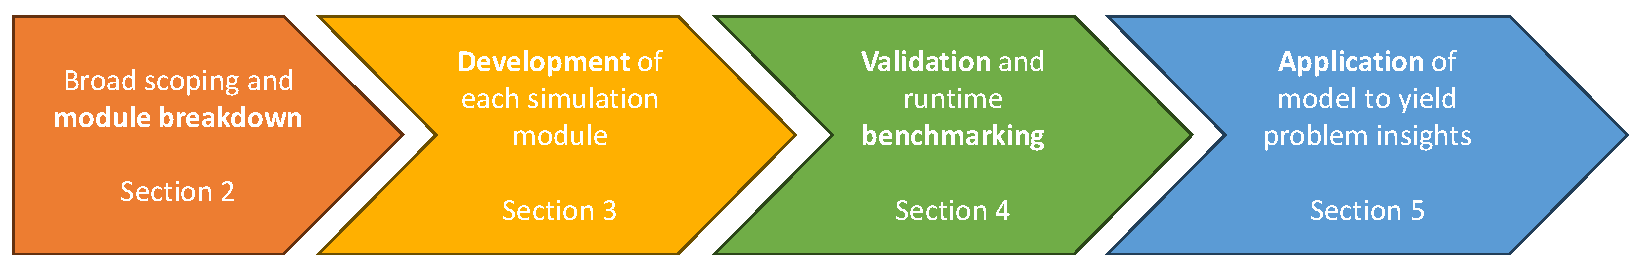
\includegraphics[width=1\linewidth]{figs/section_flow.pdf}
    \caption{Paper layout}
    \label{fig:overview-methods}
\end{figure}